% !TeX root = ../main.tex

\chapter{系统总体设计}
\label{sec:system-design}

\section{系统总体架构}

OralSage 面向口腔医学学习过程构建多模态学习平台，将专题学习、知识浏览、智能问答、数字问诊、学习画像和学习计划汇集到统一学习平台。学习者可以从学习主题、课程章节、病例训练或复习任务进入系统，在课程会话中完成资料理解、知识追问、练习检验和学习复盘，也可以在数字问诊页面完成病史采集、诊断判断和临床表达考核。知识图谱、学习画像和日历计划等可视化页面将抽象的知识结构与学习进展转化为直观信息，帮助学习者持续关注当前目标与下一步任务。

如图 \ref{fig:overall-architecture} 所示，系统以多智能体协作组织专业学习工作流。学习总控结合用户请求、课程位置和学习记录，协调课程规划、资源生成、分节讲解、课程内答疑和学习评价等智能体依次参与学习过程。课程规划确定主题结构与学习顺序，资源生成围绕课程单元准备讲义和课件，讲解答疑与练习评价在当前学习语境中接续展开。课程进度、互动结果和作答表现持续写入学习画像，并进一步影响后续学习计划，使个性化学习服务能够在同一工作流中保持连贯。

\begin{figure}[H]
  \centering
  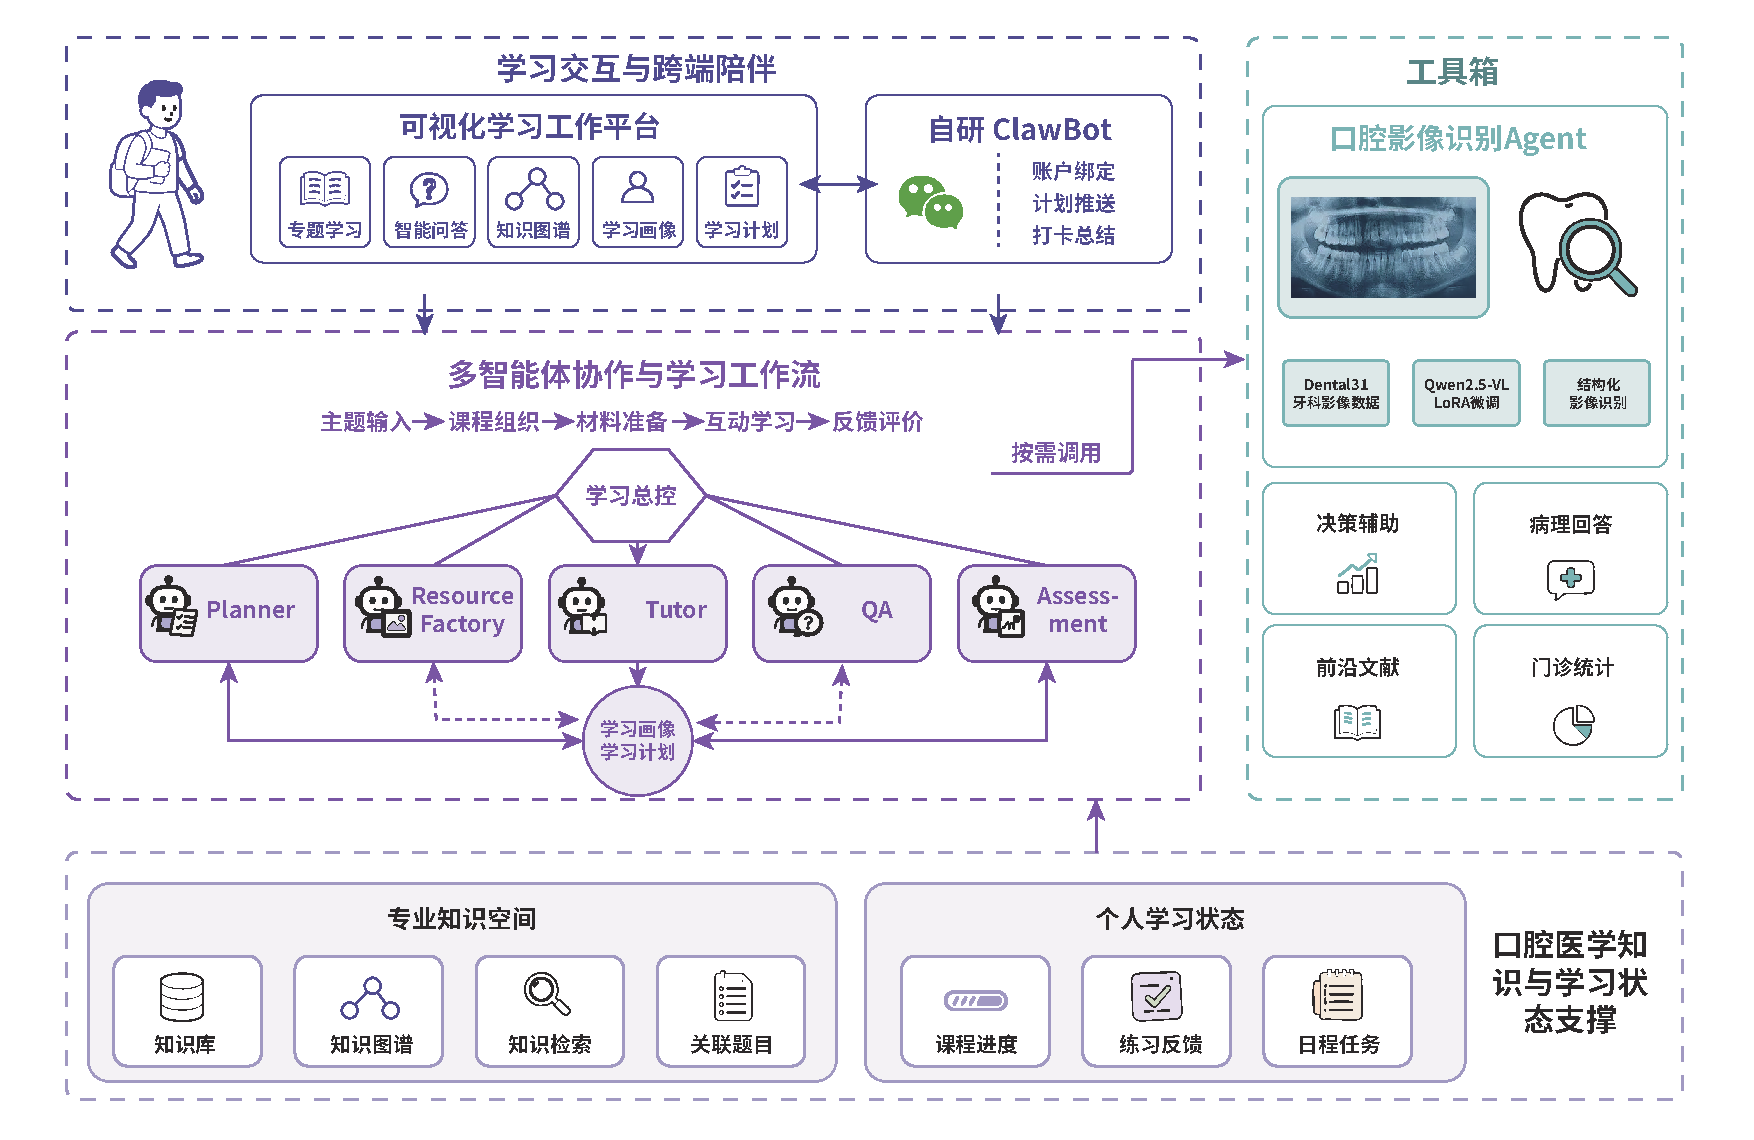
\includegraphics[width=\linewidth,height=8cm,keepaspectratio]{overall-architecture.pdf}
  \caption{OralSage 面向口腔医学个性化学习的总体架构}
  \label{fig:overall-architecture}
\end{figure}

从图\ref{fig:overall-architecture}可以看到，系统总体架构由四个相互连接的区域组成。上层是学习交互与跨端陪伴，承载专题学习、智能问答、知识图谱、学习画像、学习计划和 ClawBot 等学习入口；中层是多智能体协同与学习工作流，由学习总控协调 Planner、Resource Factory、Tutor、QA 和 Assessment 等 Agent；右侧是按需调用的专业工具箱，为影像学习、病理问答、病例分析、文献阅读、统计查询和病历文书等任务提供专项能力；下层是专业知识空间与个人学习状态，为课程规划、资源生成、教学互动和练习反馈提供知识内容、关系结构和学习记录支撑。

数字问诊通过独立的临床训练服务进入系统，患者 Agent 读取脱敏病例事实并保持多轮交流，判官 Agent 读取知识库检索证据并完成五个领域的表达评价。两类 Agent 通过诊断确认状态完成交接，问诊启动、诊断确认、分项评分和训练完成等事件写入共享学习画像。该入口与课程学习共同使用知识空间和个人学习状态，同时保留适合实时问诊的会话状态与接口边界，详细设计见第~\ref{sec:digital-consultation}章。

在知识与服务支撑层，系统将口腔医学知识库、知识图谱、专业资料片段和关联题目组织为统一的知识空间，并通过知识检索为课程规划、智能问答和练习反馈提供相关内容。当前知识底座覆盖 14 门口腔医学学科，包含 1,390 个核心条目、9,907 个知识概念、5,758 条知识关系和 3,161 道关联题目。

在此基础上，平台工具箱提供影像识别、决策辅助、门诊统计、前沿文献和病理问答等独立工具 Agent。其中，影像识别模块采用以 Qwen2.5-VL 为基座的牙科影像 LoRA 适配训练方案，为口腔影像学习和相关专业分析提供多模态能力。在跨端学习方面，自研 ClawBot 连接网页工作台与微信学习场景，支持账户绑定和学习计划推送，使学习者能够在日常沟通环境中接收任务提醒，并持续执行和跟进学习安排。

\section{专业学习闭环}

专业学习闭环描述学习者从提出主题到完成一次学习单元的过程。学习者输入学习主题后，系统结合专业知识内容和当前学习状态组织课程单元，并准备相应的讲义、课件、讲解和练习。进入课程后，学习者沿当前单元进行学习，可以在讲解过程中发起问题，也可以通过练习检验对知识内容的理解。

课程内的提问和作答反馈都会围绕当前主题和当前单元组织。QA Agent 负责补充解释，Assessment Agent 负责反馈正误、分析错因并提示需要回顾的内容。完成一个学习单元后，系统保留当前课程位置和学习结果，为继续学习或进入下一单元提供衔接。

\begin{center}
  \textbf{学习主题 $\rightarrow$ 课程与材料 $\rightarrow$ 分节学习与互动 $\rightarrow$ 练习反馈 $\rightarrow$ 学习状态 $\rightarrow$ 学习计划}
\end{center}

这一流程将主题输入、课程材料、分节学习、互动答疑和练习反馈组织为一次连续的课程会话，使学习者能够在保持课程主线的同时完成理解检验，并获得进入下一学习单元的明确衔接。

\section{学习状态驱动的持续陪伴}

OralSage 以学习画像汇集课程进度、练习反馈和学习偏好，并将这些学习状态转化为学习计划中的具体任务。学习画像通过学习活动趋势、阶段摘要和学习偏好等可视化信息呈现个人进展，学习者可以据此了解当前学习重点。完成课程或练习后，后续复习重点和日程安排随之更新，使学习记录能够自然进入下一阶段学习。

数字问诊进一步提供来自临床表达过程的细粒度信号。诊断是否正确、五个领域的分项得分和遗漏要点会更新知识节点掌握度与薄弱点，下一次病例选择再读取这些内容。学习者在课程中形成的知识状态可以影响病例训练，病例训练呈现出的表达缺口也能回到后续课程与复习安排，构成跨学习场景的动态联系。

学习计划以日历和待办承接课程内容与复习任务，学习者可以结合自己的时间安排完成、延期或调整任务。自研 ClawBot 连接网页工作台与微信学习场景，支持账户绑定和学习计划推送。学习者能够在日常沟通环境中接收任务提醒，并回到平台继续课程与计划执行，使学习陪伴覆盖更自然的使用场景。
